\documentclass{article}
\usepackage{tikz}
\usepackage[margin=0in]{geometry}
\usepackage{amsmath}
\title{}
\author{}
\date{}

\begin{document}
\begin{center}
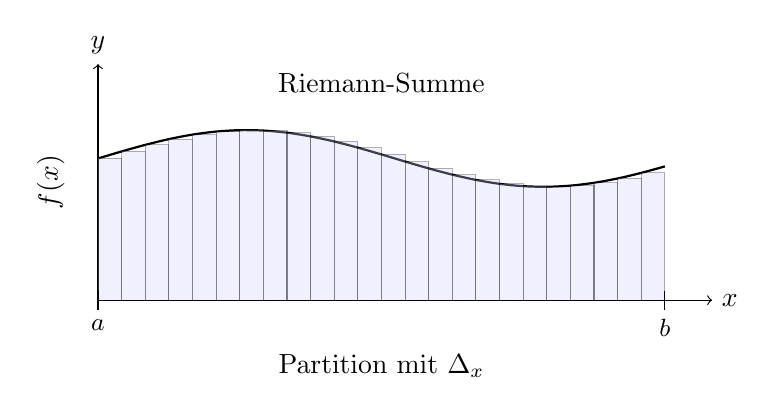
\begin{tikzpicture}[scale=1.2]
    % Define the smooth curve using a Bezier curve
    \draw[thick, domain=0:6, smooth, variable=\x] plot (\x,{1.5 + 0.3*sin(\x r)});
    
    % Draw axes
    \draw[->] (0,0) -- (6.5,0) node[right] {$x$};
    \draw[->] (0,0) -- (0,2.5) node[above] {$y$};
    
    % Draw many more rectangles with heights matching the function
    \foreach \i in {0,0.25,...,5.75} {
        \draw[fill=blue!20, opacity=0.3] (\i,0) rectangle (\i+0.25,{1.5 + 0.3*sin(\i r)});
    }
    
     \draw (0,0.1) -- (0,-0.1) node[below] {\small $a$};
     \draw (6,0.1) -- (6,-0.1) node[below] {\small $b$};
    
    % Add labels
    \node at (3,-0.7) {Partition mit $\Delta_x$};
    \node[rotate=90] at (-0.5,1.25) {$f(x)$};
    
    % Add title
    \node at (3,2.3) {Riemann-Summe};
\end{tikzpicture}
\end{center}
\begin{equation*}
\text{ Für } \Delta_x = \frac{b - a}{n}:\qquad \int_a^b f(x)\,dx = \lim_{n \to \infty} \sum_{i=0}^{n-1} f(a + i\Delta_x)\Delta_x 
\end{equation*}
\end{document}
